\documentclass{article}

\usepackage{blindtext}
\usepackage[utf8]{inputenc}
\usepackage[T1]{fontenc}
\usepackage[english,polish]{babel}
\usepackage{polski}
\usepackage{graphicx}
\usepackage{pdfpages}
\usepackage{float}
\graphicspath{ {images/} }
\usepackage{geometry}
\usepackage{color}
\usepackage{lscape}
\usepackage{subcaption}
\usepackage{xcolor}
\usepackage{listings}
\renewcommand{\lstlistingname}{Przykład}

\usepackage{caption}
\DeclareCaptionFont{white}{\color{white}}
\DeclareCaptionFormat{listing}{\colorbox{gray}{\parbox{\textwidth}{#1#2#3}}}
\captionsetup[lstlisting]{format=listing,labelfont=white,textfont=white}

\graphicspath{ {images/} }
\setlength{\topmargin}{0in}
\setlength{\textheight}{9in}
\setlength{\oddsidemargin}{.125in}
\setlength{\textwidth}{6.25in}

\setlength{\topmargin}{-.5in}
\setlength{\textheight}{9in}
\setlength{\oddsidemargin}{.125in}
\setlength{\textwidth}{6.25in}

\begin{document}


\includepdf{title_page}
\tableofcontents

\section{Opis funkcjonalno"sci projektu}
Aplikacja pozwala u"zytkownikowi na tworzenie dowolnych przepis"ow. Dane przepisy b"ed"a mog"ly by"c prywatne b"ad"z publiczne. Wszystkie przepisy publiczne b"ed"a dost"epne w API kt"ore zostanie udost"epnione. Ponadto użytkownik będzie mógł dodawać własne listy zakupowe oraz własne listy produktów. Będą one zawierały najważniejsze informację, które użytkownik będzie miał możliwo"sć posiadać podczas przygotowywania posiłków. Dodatkowo użytkownik będzie mógł ustalać i planować własne posiłki. Ponadto dzieki integracji z zewnętrznymi serwisami użytkownik będzie miał dostęp do szczegółowej analizy składników oraz będzie mógł dodać swoje posiłki do kalendarza dzięki czemu zyska lepszą kontrolę czasu jak i dostęp do powiadomień. Przyk"ladowe zapytania do API obejmują:
\begin{itemize}
	\item Wszystkie publiczne  przepisy
	\item Własne przepisy
	\item Własne listy zakupowe
	\item Własne listy posiadanych produktów
	\item Listę planowanych posiłków
\end{itemize}
Ponadto wszystkie przepisy b"ed"a mia"ly szczegółowe informacj"e o składnikach oraz o autorze danego przepisu. \par
Aplikacja mobilna jest częściowym odwzorowaniem aplikacji webowej „ReShP”. Pozwala na przeglądanie przepisów oraz list zakupowych zalogowanego użytkownika. Może on również stworzyć nową listę zakupową, lub edytować wcześniej zdefiniowaną. Aplikacja została jednak okrojona o możliwość dodawania/edycji przepisów, ze względu na zakładane nieznaczące wykorzystanie tych funkcji na urządzeniach mobilnych. \par
Dodatkową funkcją niedostępną w aplikacji webowej jest możliwość zeskanowania kodu kreskowego produktu i na jego podstawie otrzymania szczegółowych informacji o danym produkcie. Umożliwi to użytkownikowi sprawniejsze wprowadzanie zakupionych produktów do bazy danych, co wpłynie na lepsze gospodarowanie zasobami. Wszystkie dane wykorzystywane w aplikacji są przechowywane i udostępniane przez aplikację webową „ReShP” za pomocą API.

\section{Wykorzystane technologie}

\begin{itemize}
\item Python 2.7.11, Django 1.9.4
\item HTML 5
\item CSS 3
\item JavaScript
\item Java, Android
\end{itemize}

\section{Wykorzystane biblioteki}

\begin{itemize}
\item Twitter Bootstrap 3
\item Django Summernote
\item Django REST Swagger
\item Django REST Framework
\item ZXing 
\end{itemize}


\section{Wykorzystane serwisy zewnętrzne}
Aplikacja wykorzystuje trzy zewnętrzne serwisy (Edaman, Trello, Google Calendar) do pobierania oraz udostępniania danych i informacji. Korzystanie z Edamam jest obligatoryjne, jednakże korzystanie z połączenia z Trello i Google Calendar jest dobrowolne i można zadeklarować chęć korzystania z tych serwisów poprzez odpowiednie ustawienia w profilu.

\subsection{Edamam}
Edamam jest to system, kt"ory umo\.zliwia wyszukiwanie przepis"ow posiłk"ow oraz umo\.zliwa analiz"e składnik"ow w czasie rzeczywistym. W ramach działania serwisu zostały udost"epnione cztery r"o\.zne API:
\begin{itemize}
	\item Recipe Analysis and Nurtrition API
	\item Nutrition Data API
	\item Diet Recommendations API
	\item Recipe Search API
\end{itemize}

\subsection{Trello}
Trello jest to system, kt"ory umo\.zliwa tworzenie tablic wypełnion"a kartami. Ka\.zda karta mo\.ze by"c notatk"a/list"a zadań/etc... Trello API umo\.zliwa tworzenie nowych tablic/notatek jak i dodawanie nowych, bad"z modyfikowanie czy usuwanie starych. Przykładowe zapytanie zwr"ocenia informacji o karcie:

\subsection{Google Calendar API}
Google Calendar jest to system, który umożliwia tworzenie wydarzeń wraz z przypomnieniami.

\section{Diagram ERD}

\begin{landscape}
\begin{figure}[!ht]
  \centering
    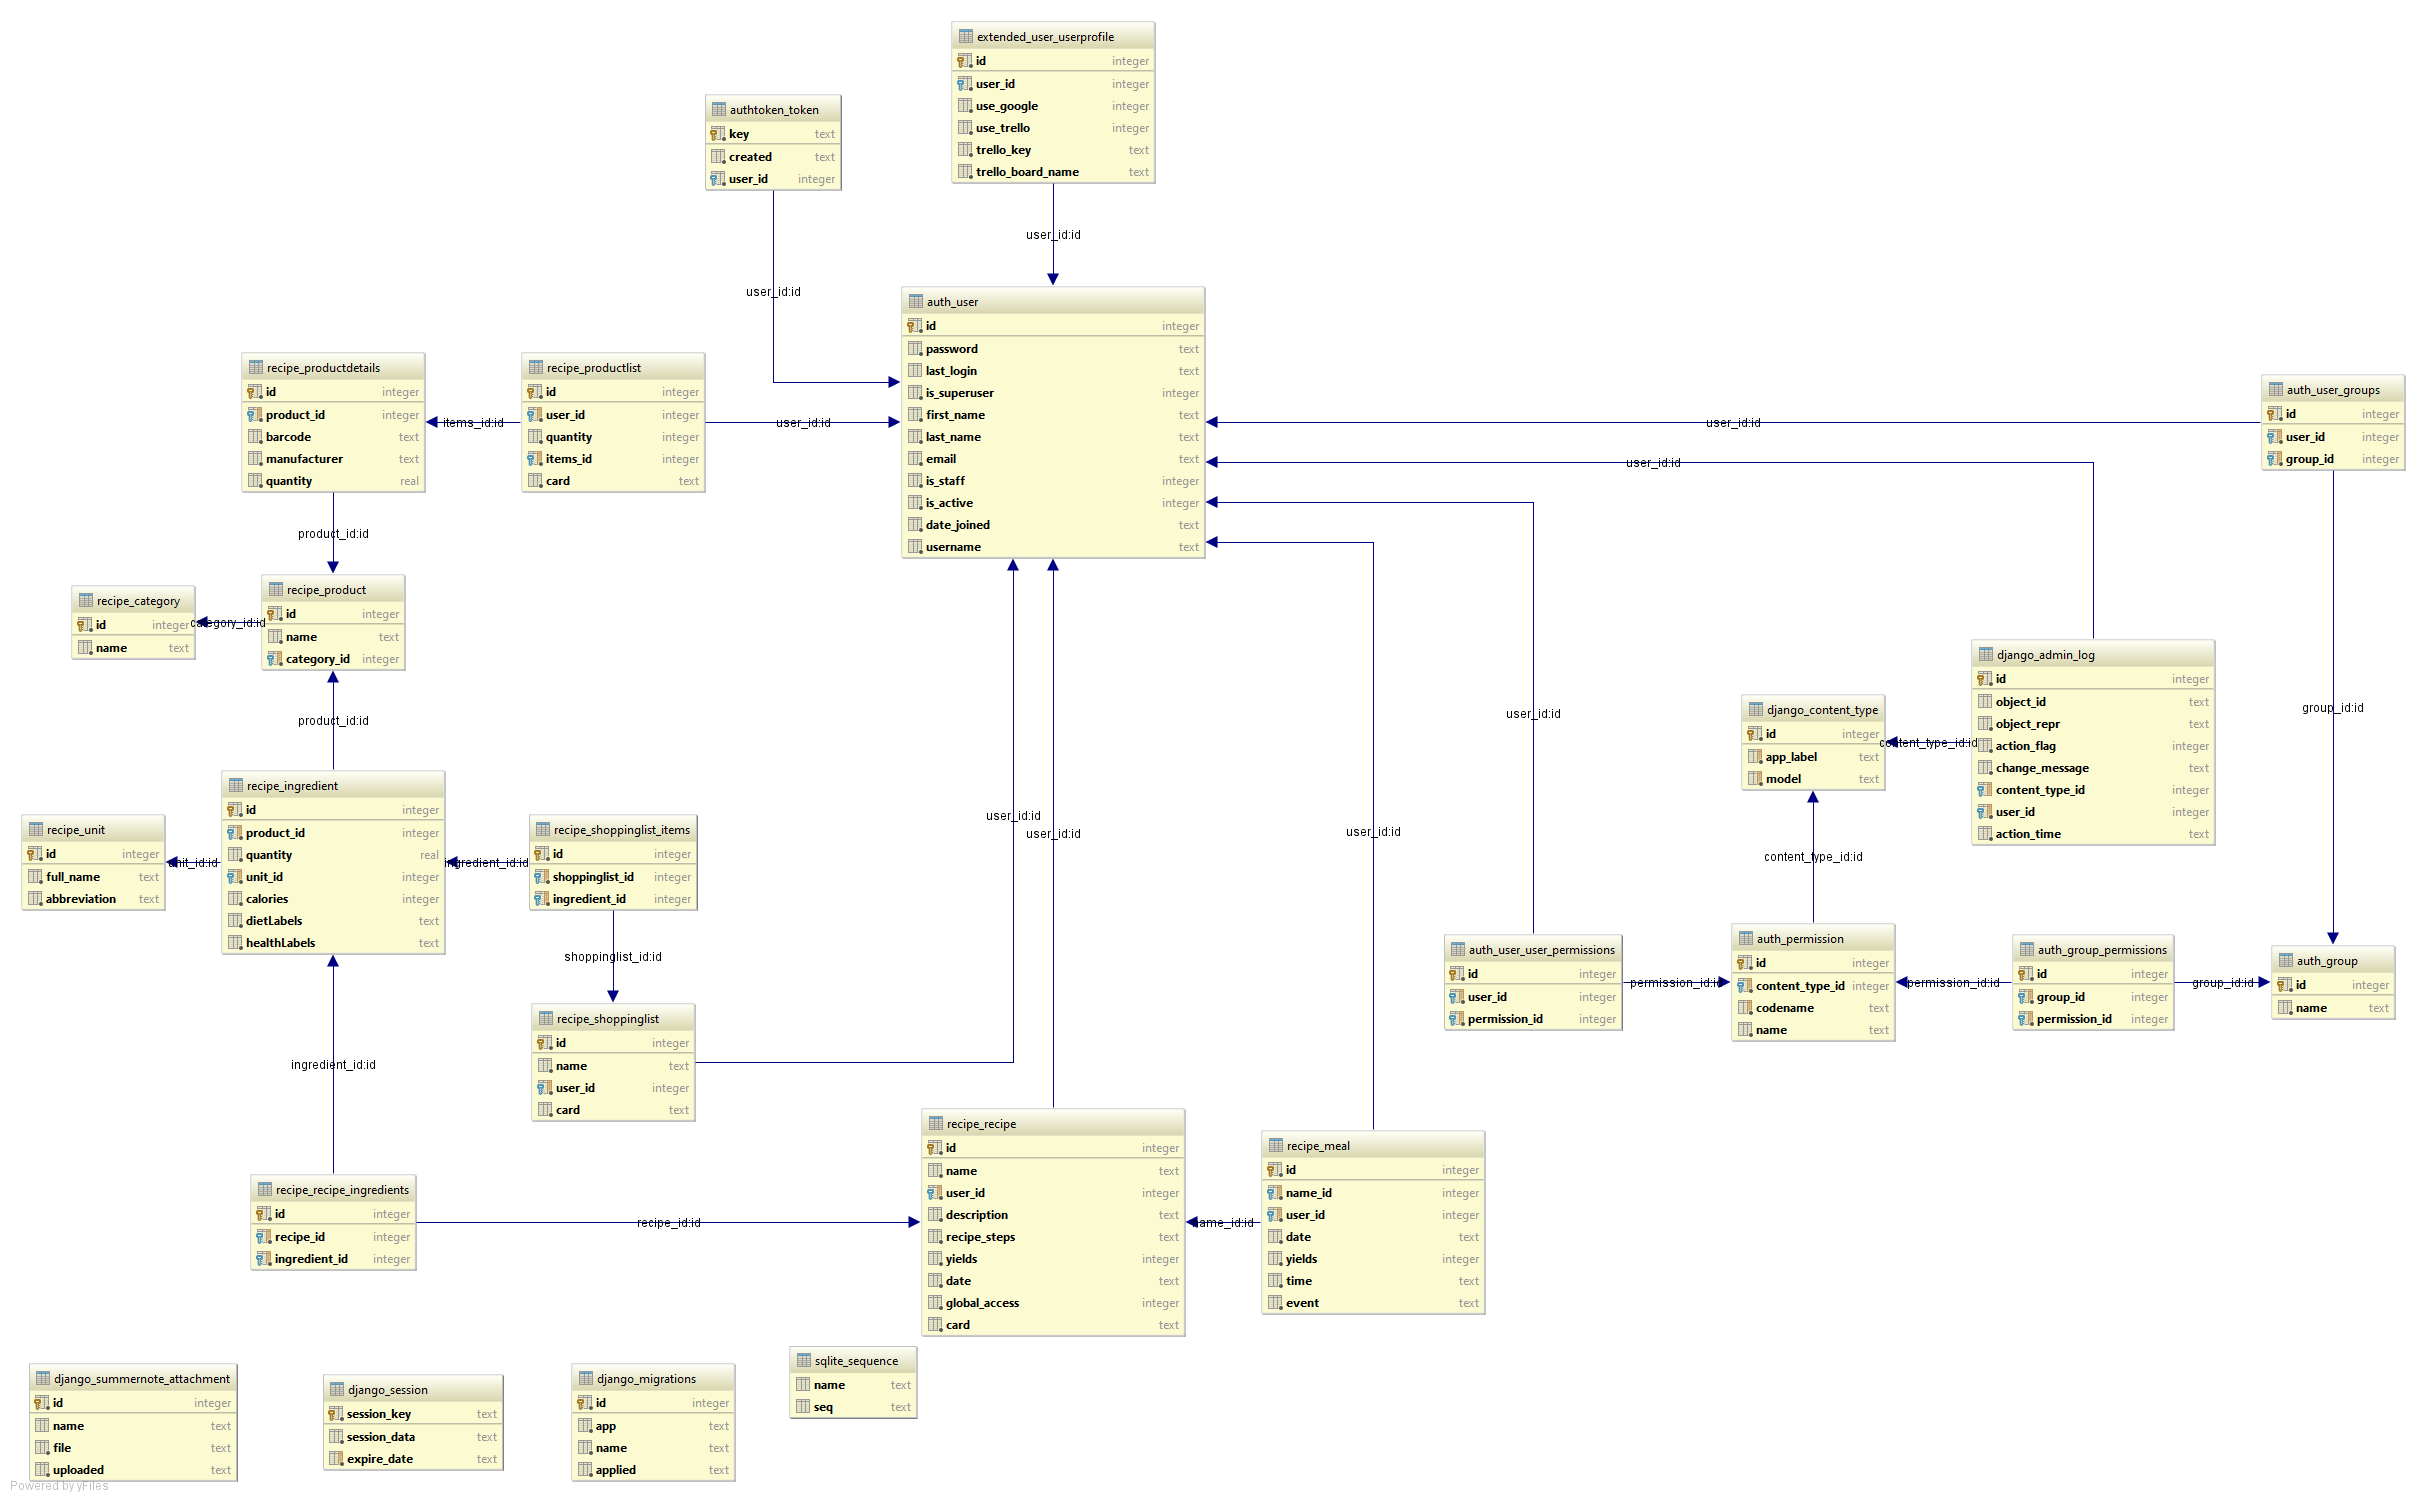
\includegraphics[width=1.5\textwidth]{erd}\par\vspace{1cm}
  \caption{Diagram ERD}
\end{figure}
\end{landscape}

\section{Diagramy BPMN}
\section{Wygląd interfejsu użytwkonika}
Po uruchomieniu aplikacji użytkownik ma do wyboru jedną z czterech opcji: przej"scie na stronę główną, przegląd publicznie udostępnionych przepisów, zalogowanie się, bądź zarejestrowanie się (Rysunek 2).
\begin{figure}[!ht]
  \centering
    
\includegraphics[]{reshp1}\par\vspace{1cm}
  \caption{Menu dla niezalogowanego użytkownika}
\end{figure}

Jeżeli użytkownik wybierzę opcję rejestracji to pojawi się nowe okno, gdzie użytkownik zostanie poproszony o podanie: nazwy użytkownika, adres email oraz hasło dostępowe (Rysunek 3).
\begin{figure}[!ht]
  \centering
    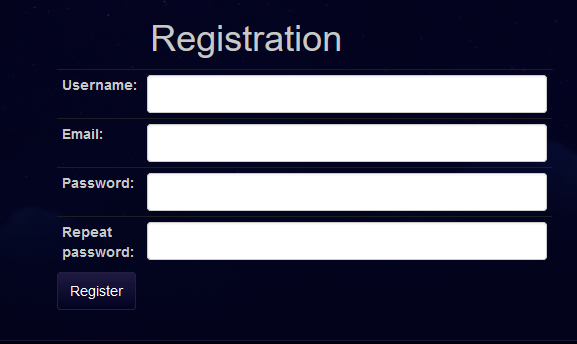
\includegraphics[width=0.5\textwidth]{reshp2}\par\vspace{1cm}
  \caption{Rejestracja nowego użytkownika}
\end{figure}

Jeżeli użytkownik wybierzę opcję logowania to poajwi się nowe okno, gdzie użytkownik zostanie poproszony o podanie: nazwy użytkownika oraz hasła dostęppowego (Rysunek 4).
\begin{figure}[!ht]
  \centering
    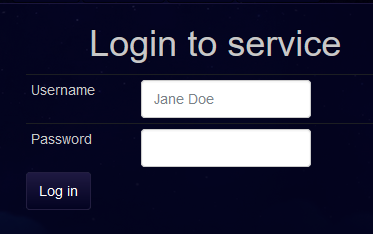
\includegraphics[width=0.5\textwidth]{reshp3}\par\vspace{1cm}
  \caption{Logowanie do aplikacji}
\end{figure}

Po zalogowaniu dla użytkownika pojawiają sie nowe opcję do wyboru. Może wybrać jedną z następujących akcji: przeglądanie przepisów, dodawanie nowego przepisu, przeglądanie posiłków, dodawanie nowego posiłku, przeglądanie listy zakupowej, dodawanie nowej listy zakupowej, przeglądanie produktów, dodawanie nowych produktów, uaktualnienie profilu, bądź wylogowanie się (Rysunek 5).
\begin{figure}[!ht]
  \centering
    
\includegraphics[width=1\textwidth]{reshp4}\par\vspace{1cm}
  \caption{Menu dla zalogowanego użytkownika}
\end{figure}

Jeżeli użytkownik wybierzę opcję uaktualnienia profilu to może on wypełnić potrzebne informację do korzystania z serwisów zewnętrznych (Rysunek 6).
\begin{figure}[!ht]
  \centering
    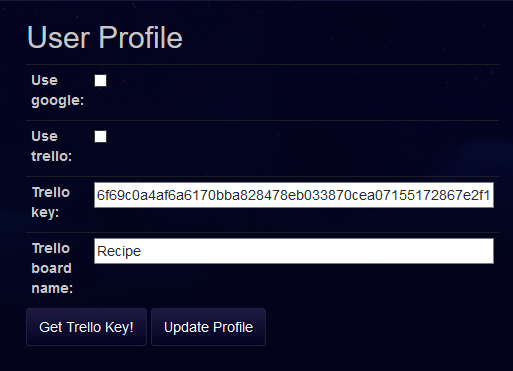
\includegraphics[width=0.5\textwidth]{reshp5}\par\vspace{1cm}
  \caption{Profil uiżytkownika}
\end{figure}

Jeżeli użytkownik wybierzę opcję dodawania przepisu to pojawi się nowe okno w którym będzie mógł uzupełnić informację o nowym przepisie. Do wypełenienia ma: nazwę przepisu, krótki opis, ilo"sć porcji, opis jak wykonać przepis oraz informację o składnikach takich jak: nazwa składnika, ilo"sć składnika, kategorię składnika oraz jednostkę mierzenia (Rysunek 7).
\begin{figure}[!ht]
  \centering
    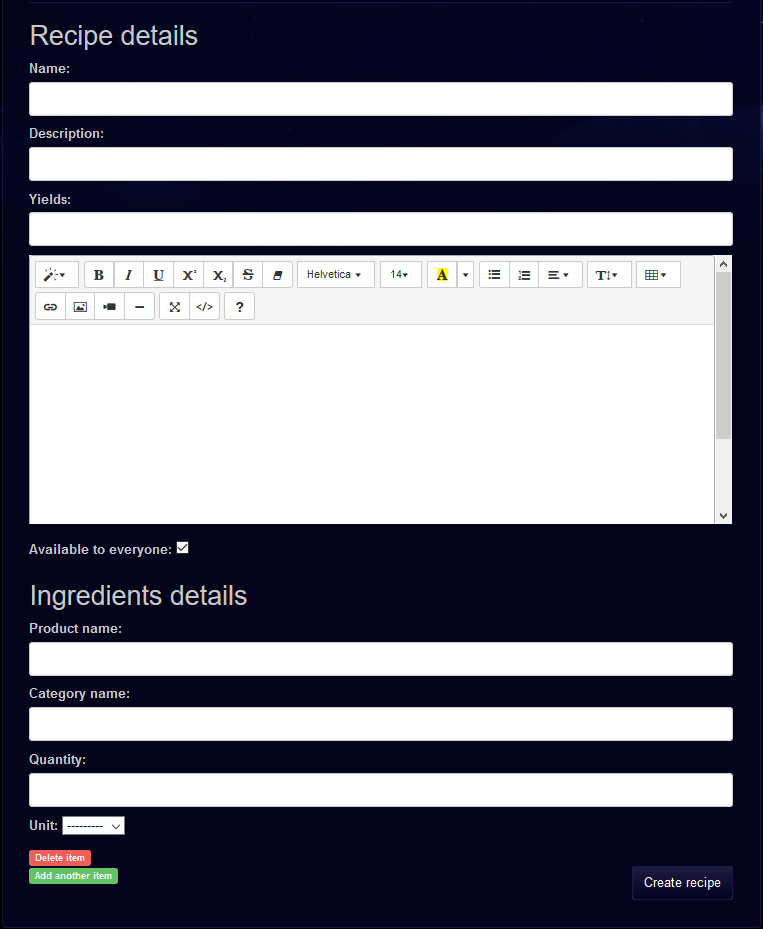
\includegraphics[width=0.5\textwidth]{reshp6}\par\vspace{1cm}
  \caption{Rejestracja nowego użytkownika}
\end{figure}

\newpage
Jeżeli użytkownik wybierzę opcję dodawanie posiłku to pojawi się nowe okno w którym będzie mógł uzupełnić informację o nowym posiłku. Do wypełnienia ma: nazwę dania, które będzie podawane, datę posiłku, godzinę posiłku oraz liczbę porcji (Rysunek 8).
\begin{figure}[!ht]
  \centering
    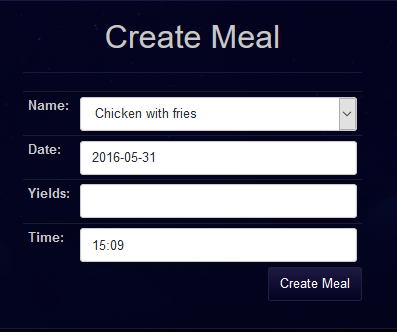
\includegraphics[width=0.5\textwidth]{reshp7}\par\vspace{1cm}
  \caption{Dodawanie posiłku}
\end{figure}

Jeżeli użytkownik wybierzę opcję dodawanie listy zakupowej, to pojawi się nowe okno, w którym bedzie mógł uzupełnić informację o nowej li"scie zakupowej. Do wypełnienia ma: nazwę listy zakupowej oraz informację o produktach: nazwa produktu, kategoria produktu, ilo"sć produktu oraz jednostka w jakiej produkt jest mierzony (Rysunek 9a). 
\begin{figure}[!ht]
  \centering
    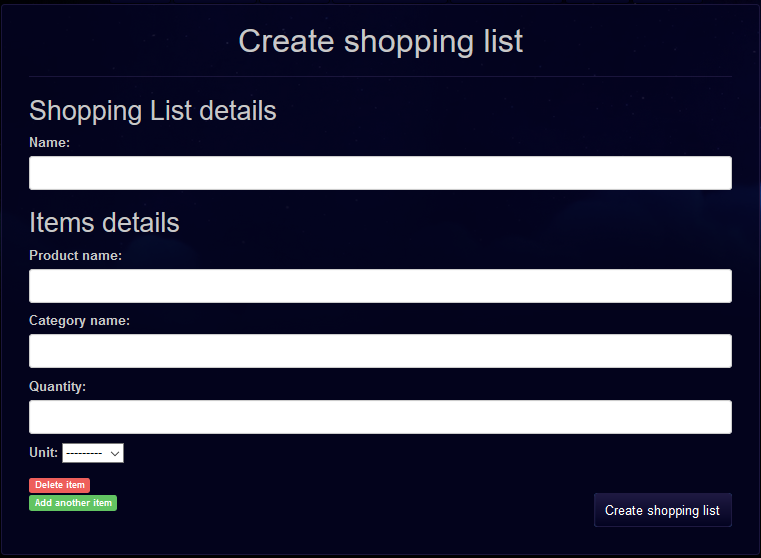
\includegraphics[width=0.5\textwidth]{reshp8}\par\vspace{1cm}
  \caption{Dodawanie nowej listy zakupowej}
\end{figure}

Jeżeli użytkownik wybierzę opcję dodawanie listy zakupowej to pojawi się nowe okno, w którym będzie mógł uzupełnić informację o nowym produkcie. Do wypełnienia ma: nazwę produktu, kategorię produktu, ilo"sć produktu, producenta, ilo"sć w opakowaniu oraz kod kreskowy (Rysunek 10a).Jeżeli jest to robione za pomocą telefonu komórkowego to użytkownik ma do dyspozycji czytnik kodu kreskowego (Rysunek 10b), który zeskanuje i odnajdzie odpowiednie dane, które będziemy mogli wykorzystać w formularzu (Rysunek 10c).
\begin{figure}[!ht]
  \centering
\begin{subfigure}{.3\textwidth}
  \centering
   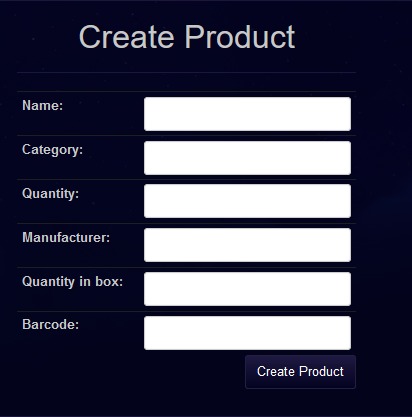
\includegraphics[width=1\textwidth]{reshp9}\par\vspace{1cm}
  \caption{Formularz dodawanie listy zakupowej}
  \label{fig:sub1}
\end{subfigure}%
\begin{subfigure}{.3\textwidth}
  \centering
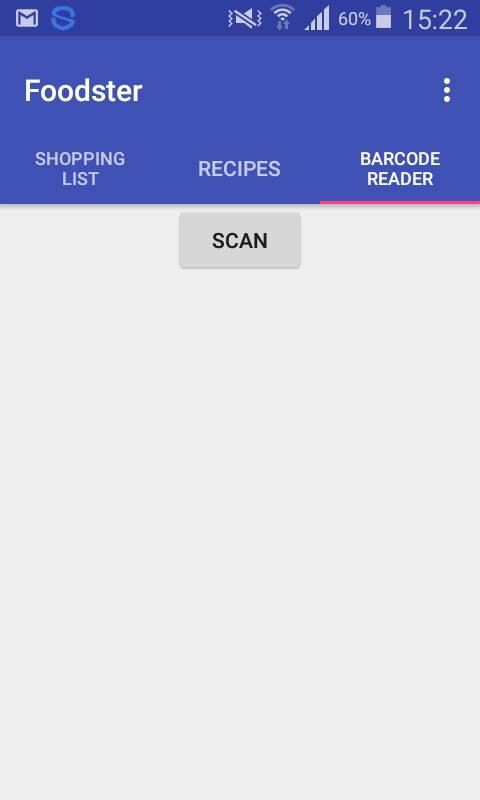
\includegraphics[width=0.8\textwidth]{barcode1}\par\vspace{1cm}
  \caption{Opcja skanowania produktu z poziomu telefonu}
  \label{fig:sub1}
\end{subfigure}%
\begin{subfigure}{.3\textwidth}
  \centering
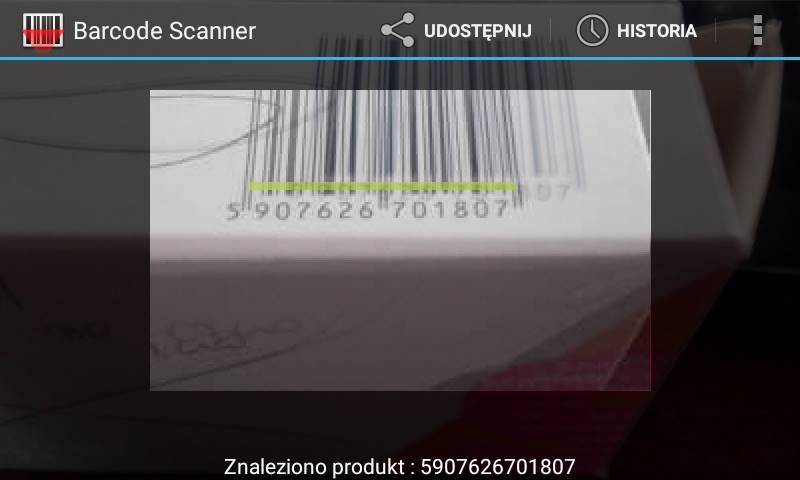
\includegraphics[width=1\textwidth]{barcode3}\par\vspace{1cm}
  \caption{Skanowanie produktu}
  \label{fig:sub1}
\end{subfigure}%
  \caption{Dodawanie nowego produktu}
\end{figure}

Jeżeli użytkownik wybierzę opcję przeglądania przepisu to wy"swietli mu się szczegółowy opis przepisu, który wprowadził, wraz z szczegółowym opisem poszczególnych składników zawierające takie dane jak: kalorie, dietetyczne etykiety, czy zdrowotne etykiety (Rysnuek 11).
\begin{figure}[!ht]
  \centering
   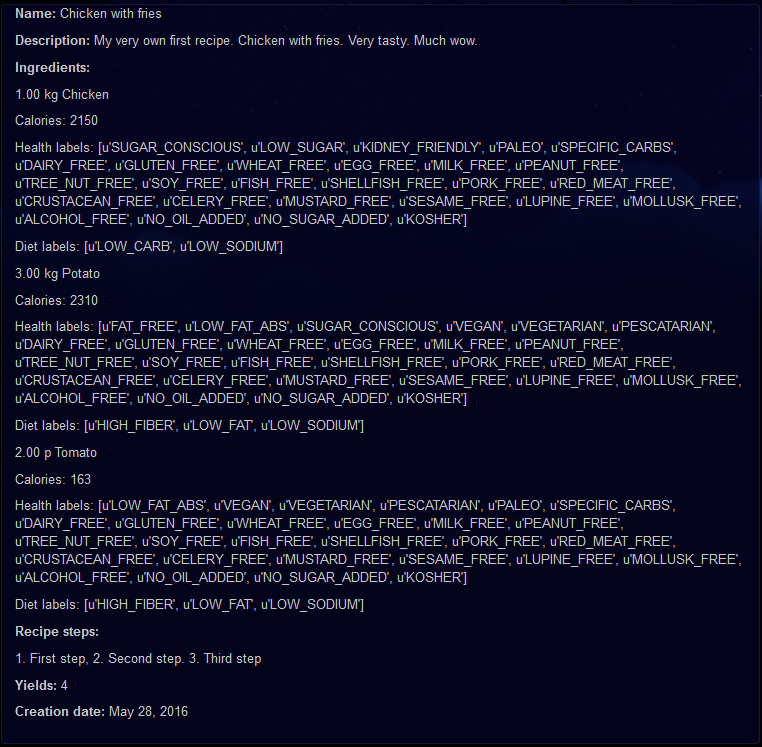
\includegraphics[width=1\textwidth]{reshp10}\par\vspace{1cm}
  \caption{Wy"swietlanie przepisu}
\end{figure}
\newpage
Jeżeli użytkownik wybierzę opcję przeglądania posiłku to wy"swietli mu się szczegółowy opis posiłku, który wprowadził, wraz z szczegółowym opisem przepisu, który został powiązany z danym posiłkiem (Rysunek 12).
\begin{figure}[!ht]
  \centering
   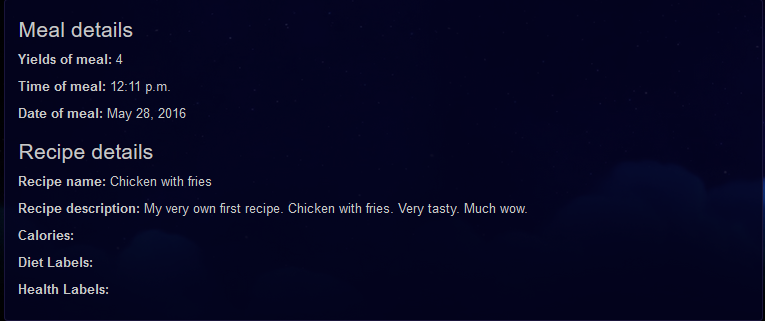
\includegraphics[width=1\textwidth]{reshp11}\par\vspace{1cm}
  \caption{Wy"swietlanie posiłku}
\end{figure}

Jeżeli użytkownik wybierzę opcję przeglądania listy zakupowej, to wy"swietli mu się szczegółowy opis listy (Rysunek 13).
\begin{figure}[!ht]
  \centering
    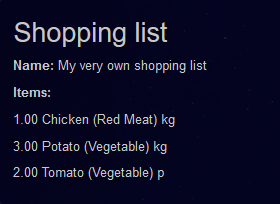
\includegraphics[]{reshp12}\par\vspace{1cm}
  \caption{Wy"swietlanie listy zakupowej}
\end{figure}
\newpage
Jeżeli użytkownik wybierzę opcję przeglądania produktu, to wy"swietli mu się szczegółowy opis danego produktu (Rysunek 14).
\begin{figure}[!ht]
  \centering
    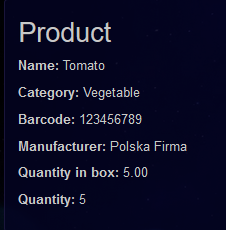
\includegraphics[]{reshp13}\par\vspace{1cm}
  \caption{Wy"swietlanie produktu}
\end{figure}

\section{Wnioski}

\end{document}